% fig-copies.tex: recovery from a second copy, a retrieve after a rollback at one storage server (draft of 6 Nov 2026).
% Build from this folder:  pdflatex fig-copies.tex
% Source: section 4.8 ("The design") and Table 4.4, row "stale (rolled back) | current | honest": accepted from D2, D1 repaired.
% Status of what is drawn: designed; the mechanism demonstrated at one provider (Table 6.6).
\documentclass[tikz,border=4pt,11pt]{standalone}
% style.tex: what the four diagrams share (colours, fonts, the look of a party, a message, a note).
% The one accent colour is the blue of the latency charts; it always means "the head", the thing this thesis adds.
% Everything else is black or grey, so the figures still read when printed in black and white.
\usepackage[T1]{fontenc}
\usepackage{mathptmx}
\usetikzlibrary{positioning,calc,arrows,fit,backgrounds}
\definecolor{head}{HTML}{2A78D6}
\definecolor{ink}{HTML}{0B0B0B}
\definecolor{inktwo}{HTML}{52514E}
\definecolor{soft}{HTML}{F0EFEC}
\definecolor{rule}{HTML}{C3C2B7}
\tikzset{
  every picture/.style={font=\small, >=latex},
  party/.style={draw=ink, fill=soft, rounded corners=2pt, minimum width=3.4cm, minimum height=0.8cm, align=center, font=\small\bfseries},
  box/.style={draw=ink, fill=soft, rounded corners=2pt, minimum width=3.9cm, minimum height=1.9cm, align=center},
  quiet/.style={draw=rule, text=inktwo},
  life/.style={draw=rule, line width=0.9pt},
  msg/.style={->, draw=ink, line width=0.7pt},
  rep/.style={->, draw=ink, line width=0.7pt, dashed},
  hmsg/.style={->, draw=head, line width=1.2pt},
  hrep/.style={->, draw=head, line width=1.2pt, dashed},
  bad/.style={->, draw=ink, line width=1.2pt, dashed},
  lab/.style={font=\footnotesize, inner sep=3pt, text=ink},
  act/.style={font=\footnotesize, align=left, text=ink, fill=white, draw=rule, rounded corners=1.5pt, inner sep=3pt},
  outcome/.style={font=\footnotesize, align=center, text=ink, fill=white, draw=ink, rounded corners=1.5pt, inner sep=4pt},
  side/.style={font=\footnotesize\itshape, align=left, text=inktwo},
  band/.style={fill=soft, draw=rule, rounded corners=2pt, minimum height=0.7cm, font=\footnotesize, text=inktwo},
  holds/.style={font=\footnotesize, text=inktwo, fill=white, draw=rule, rounded corners=1.5pt, inner sep=2.5pt},
}

\begin{document}
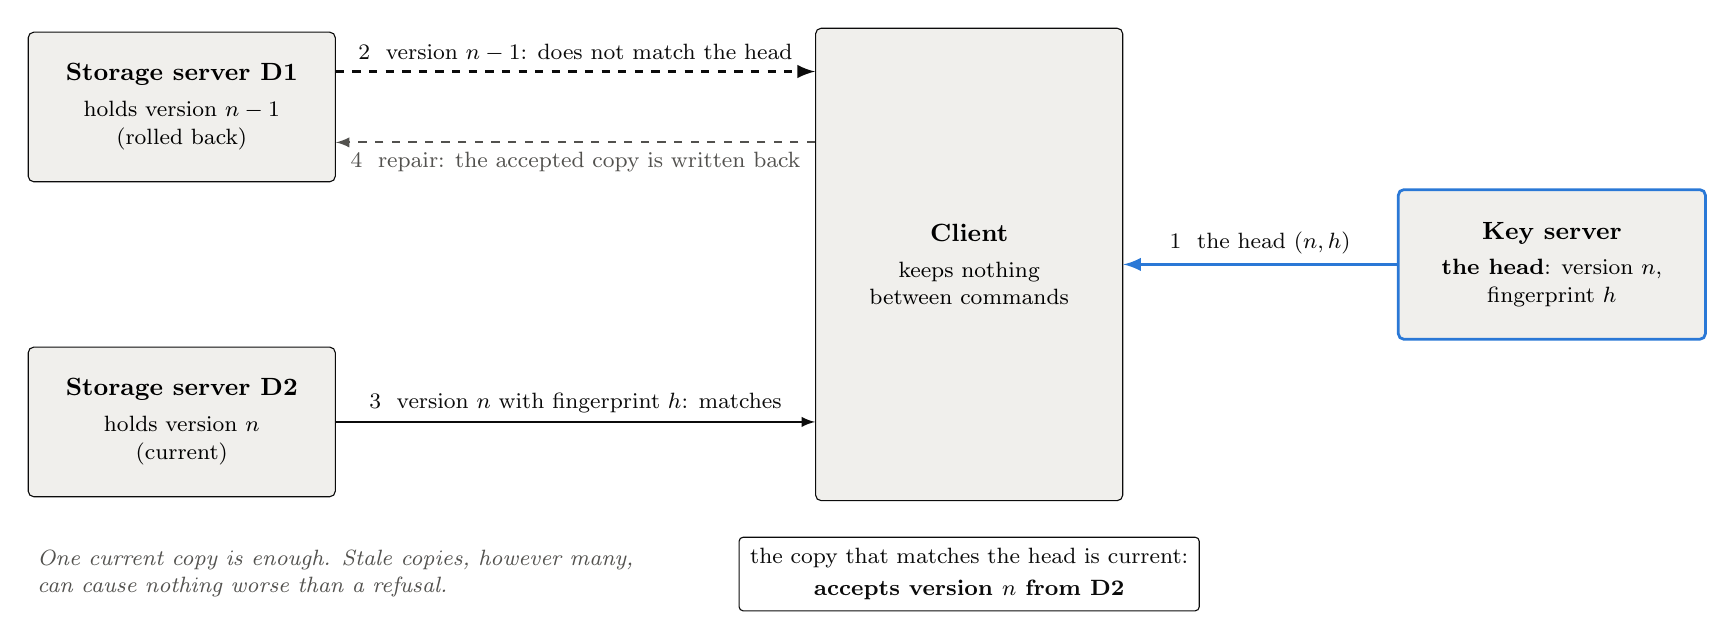
\begin{tikzpicture}
\node[box] (D1) at (0,2.0)    {\textbf{Storage server D1}\\[2pt]\footnotesize holds version $n-1$\\[-1pt]\footnotesize (rolled back)};
\node[box] (D2) at (0,-2.0)   {\textbf{Storage server D2}\\[2pt]\footnotesize holds version $n$\\[-1pt]\footnotesize (current)};
\node[box, minimum height=6.0cm] (C) at (10.0,0) {\textbf{Client}\\[2pt]\footnotesize keeps nothing\\[-1pt]\footnotesize between commands};
\node[box, draw=head, line width=1.0pt] (K) at (17.4,0) {\textbf{Key server}\\[2pt]\footnotesize \textbf{the head}: version $n$,\\[-1pt]\footnotesize fingerprint $h$};
% 1: the head
\draw[hmsg] (K.west) -- node[lab, above] {1\ \ the head $(n, h)$} (C.east);
% 2: the stale copy from D1
\draw[bad] ([yshift=0.45cm]D1.east) -- node[lab, above] {2\ \ version $n-1$: does not match the head} ([yshift=0.45cm]D1.east -| C.west);
% 4: repair of D1
\draw[->, draw=inktwo, line width=0.7pt, dashed] ([yshift=-0.45cm]D1.east -| C.west) -- node[lab, below, text=inktwo] {4\ \ repair: the accepted copy is written back} ([yshift=-0.45cm]D1.east);
% 3: the current copy from D2
\draw[msg] (D2.east) -- node[lab, above] {3\ \ version $n$ with fingerprint $h$: matches} (D2.east -| C.west);
\node[outcome, below=0.45cm of C] (o) {the copy that matches the head is current:\\[2pt] \textbf{accepts version $n$ from D2}};
\node[side, anchor=north west] at ([yshift=-0.55cm]D2.south west) {One current copy is enough. Stale copies, however many,\\ can cause nothing worse than a refusal.};
\end{tikzpicture}
\end{document}
